\documentclass[UTF8,12pt,a4paper,fontset=none]{ctexart}
\setCJKmainfont[ItalicFont={Noto Serif CJK SC},SlantedFont={Noto Serif CJK SC}]{Noto Serif CJK SC}
\setCJKsansfont{Noto Sans CJK SC}
\setCJKmonofont{Noto Sans Mono CJK SC}
\usepackage{amsmath,amssymb,booktabs,geometry,graphicx,array,tabularx}
\usepackage{fvextra}
\usepackage[section]{placeins}
\usepackage[hidelinks]{hyperref}
\geometry{left=2.5cm,right=2.5cm,top=2.5cm,bottom=2.5cm}
\newcommand{\keywords}[1]{\par\medskip\noindent\textbf{关键词：}#1}
\setlength{\emergencystretch}{2em}
\setcounter{topnumber}{3}
\renewcommand{\topfraction}{0.9}
\renewcommand{\textfraction}{0.08}
\renewcommand{\floatpagefraction}{0.8}
\begin{document}
\pagestyle{plain}
\begin{center}
{\LARGE\bfseries 变物性药材烘干的守恒建模与全域判定}
\end{center}
\begin{abstract}
针对圆柱形药材烘干过程中温度与水分变化不同步、后期扩散减慢以及收缩后的终点判定问题，建立理想化、有效参数的一维径向传热传质模型。以干基含水率描述水分状态，以径向最大含水率低于0.15作为烘干完成条件，并用平均含水率和表面含水率辅助分析内部差异。

对题给环境和半径数据作分段线性插值，4小时后环境固定为50摄氏度和0.05 kg/kg。固定域采用守恒有限体积法离散热湿耦合方程，结合表面加密网格与隐式BDF方法求解。收缩域采用随体坐标，由干质量守恒推导干基水分方程，在同一离散框架下计算变化半径对传递过程的影响。

问题一在0.50小时的中心、表面温度分别为33.5753、36.7856摄氏度，含水率分别为2.5500、1.5102。问题二在3小时的径向温差为0.1169摄氏度，中心、表面含水率仍分别为1.7662、1.0081，表明水分均匀化明显滞后于升温。问题三、四的越阈时间分别为57.4728、51.0908小时，问题四终点半径为1.2000厘米。四问均按题目要求输出结果，收缩后域外位置留空。

问题四相对问题三的时间缩短11.1043\%。保持问题四物性、将半径固定为初值时，对照时间为129.8449小时；同物性条件下，收缩使时间减少60.6524\%。这两个降幅分别描述总体差异和给定物性下的几何影响。固定域与移动域解析算例、水分平衡以及空间和时间加密检验共同支持所用离散方法，最终采用640个径向区间计算题目结果。
\keywords{药材烘干；热湿耦合；守恒有限体积；移动边界；全域阈值}
\end{abstract}
\clearpage
\section{问题重述与总体分析}
\subsection{研究对象、变量和四问的递进关系}
烘干过程的直接目标是降低药材内部水分，而不是仅使外表面变干或达到环境温度。题设药材初始为长25厘米、半径2厘米的圆柱，初始温度均匀为28摄氏度，初始水分为每千克干物质含2.55千克水。后一个量是干基含水率，以下记为$C$，并始终保留其质量基准。数值$C=2.55$不意味着湿物料中水的质量分数大于一；对应的湿基质量分数为$C/(1+C)$。题设物性中的这一比值与状态变量本身不能混用，终止阈值0.15也作用于干基变量。

问题一要求利用给定环境时间序列及常热物性，计算前1800秒内部温度和水分的径向分布，并按指定时空分辨率输出。它构成整个模型的基础情景：几何不变，热传导不受水分反馈影响，而水分扩散系数随含水率变化。问题二引入温湿相关物性，温度通过扩散系数影响脱水，水分又通过有效热容量和导热率影响升温。因而必须求解两组状态的联立初边值问题，而不能先独立求温度、再以固定温度计算全部干燥过程。

问题三沿用问题二的物性与固定半径，把时间范围延伸到所有位置满足含水率要求。此时任务的重点由给定时刻的场分布转向首次满足全域条件的时间。问题四进一步给出随时间变化的实测半径及另一组物性。其难点不仅是扩散距离缩短，还包括计算域移动、干基变量的输运解释，以及固定物理位置是否仍在药材内部。本文分别输出名义结果和同物性几何对照，避免将多因素差异解释成单因素效应。

表\ref{tab:task-map}概括四问的递进关系。四问共用径向守恒离散与边界符号，分别改变物性、输出范围及几何。问题二、三共享同一个从初态出发的完整解，问题四则同时改变物性与几何；这一结构决定了哪些结果可以直接比较、哪些差异需要另设对照。

\begin{table}[htbp]\centering\small
\caption{四问的模型变化、求解目标与结果对应}\label{tab:task-map}
\begin{tabularx}{\linewidth}{cXXl}
\toprule
问题 & 物性与几何 & 核心求解目标 & 正文数值表\\
\midrule
一 & 常热物性，$D(C)$，固定半径 & 前1800秒温度、水分径向场 & \ref{tab:paper1}、\ref{tab:paper2}\\
二 & 温湿相关物性，固定半径 & 全过程耦合场及前三小时摘录 & \ref{tab:paper3}、\ref{tab:paper4}\\
三 & 完全沿用问题二 & 全域含水率首次越阈及整秒终点 & \ref{tab:paper5}\\
四 & 另一组物性，给定$R(t)$ & 移动域越阈、实际表面及域内输出 & \ref{tab:paper6}\\
\bottomrule
\end{tabularx}
\end{table}

本文的处理重点是三处一致性：用共享面通量保证离散水分收支；用干基变量与随体坐标保证收缩运动的解释一致；用最大值事件及同物性对照保证终点判定和几何归因一致。它们是经典方法针对本题的组合与细化，不以算法名称的新颖性替代数值证据。题目未提供内部观测，因此不进行参数回归；环境、半径是输入，内部场与终点是模型输出。

\subsection{空间非均匀性与模型选择}
圆柱侧面与环境发生热量和水分交换，中心没有跨轴线的净通量。升温时，热量从表面向内传递；脱水时，内部水分向表面迁移。这两种过程的特征时间未必相同。因此，截面平均温度接近环境不能推出中心已干燥，表面达到含水阈值也不能代替全截面判定。本文保留径向坐标，以全域最大含水率作为终点变量，同时保存体积权均值与表面值解释空间差异。

本文研究轴向与周向均匀、径向允许非均匀的一维理想场。轴向和周向不设独立状态，题给长度保持不变。下文“全域”均指所定义的径向场，不将有限圆柱的端部效应另设为待求机制，也不以长径比推断未计算的三维误差。

已有圆柱干燥研究比较过有限外部传质阻力与表面直接给定状态的边界形式\cite{silva2014turmeric}。题目给定热、质传递系数，因此本文保留Robin边界，不把表面温度强制等于空气温度，也不把表面含水率强制等于环境记录。变物性耦合干燥可用隐式有限体积方法求解\cite{silva2014coupling}；本文采用该类方法的守恒通量思想，但所有材料函数均取自题目，不迁移文献中其他食品的经验参数。

\section{数据盘点、单位与边界重建}
\subsection{全量输入检查}
附件1含241条环境记录，时间从0到14400秒，等间隔60秒。温度从28摄氏度升至接近50摄氏度，水分记录从0.01963升至约0.05。附件2含145条半径记录，时间从0到259200秒，等间隔1800秒，半径单位为厘米。两份数据均无缺失值、非有限数值或重复时间，时间严格递增；原始半径非增，具有53个不同数值和92次相邻重复。这些重复反映测量分辨率及后期平台，不是需要删除的重复记录。

表\ref{tab:data}给出数据的作用和处理约定。计算中使用全部241条环境记录和全部145条半径记录，不为得到平滑曲线删除局部波动。热湿状态计算采用国际单位制，半径进入微分方程前除以100，时间保持秒；展示时才转换为厘米或小时。这里的单位转换尤其重要，因为扩散特征时间与半径平方成正比，误将厘米当米会使几何尺度发生严重偏差。

\begin{table}[htbp]\centering\small
\caption{原始附件与输出模板的数据合同}\label{tab:data}
\begin{tabularx}{\linewidth}{lrrX}
\toprule
对象 & 记录数 & 时间范围/h & 角色与处理\\
\midrule
附件1 & 241 & 0--4 & 温度与有效平衡含水率边界；全量线性插值\\
附件2 & 145 & 0--72 & 实测半径；厘米转米，保留全部平台记录\\
结果模板1、2 & 两工作表 & 见正文 & 温度、水分分别输出；每秒和每0.1厘米\\
结果模板3、4 & 单工作表 & 至严格终点 & 含水率每60秒输出，并补入最终整秒\\
\bottomrule
\end{tabularx}
\end{table}

图\ref{fig:q1-environment}展示全部环境输入。早期环境显著变化，不能用最终50摄氏度替代整个过程；后期小幅波动也不构成内部状态的实验验证。图中的有效平衡含水率表示本文约定的边界数值$C_e=W_a$，其中$W_a$为附件水分记录。该映射是有效传质模型的定义，不表示空气与固体的质量基准相同，也不声称由本题数据识别出了真实吸附平衡关系。

\begin{figure}[htbp]\centering
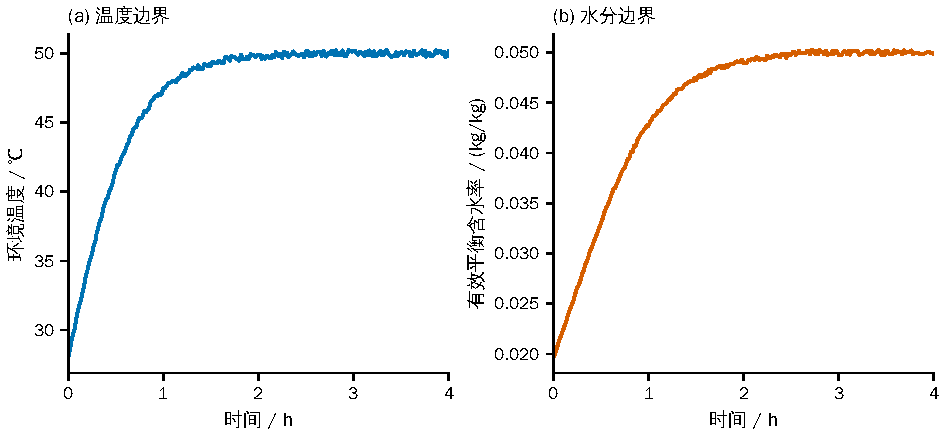
\includegraphics[width=\linewidth]{figures/raw_q1_environment.pdf}
\caption{环境边界输入：全部241条记录分别重建温度与有效边界$C_e$，两种量采用独立纵轴面板。}\label{fig:q1-environment}
\end{figure}

\subsection{分段插值与四小时后的名义环境}
记环境温度为$\theta_\infty(t)$，有效平衡含水率为$C_e(t)$。对任意相邻实测时刻$t_j,t_{j+1}$，采用式\eqref{eq:interp}重建二者。线性插值保留原始端点，避免高阶多项式在边界波动处产生未经数据支持的过冲，也无需选择平滑强度或拟合阶数。插值函数连续但导数可以在记录时刻改变，这是对离散采样信息的明确使用，而不是宣称真实环境只有分段线性变化。

\begin{equation}\label{eq:interp}
b(t)=b_j+\frac{t-t_j}{t_{j+1}-t_j}(b_{j+1}-b_j),
\quad t_j\leq t\leq t_{j+1},\quad
b\in\{\theta_\infty,C_e\}.
\end{equation}

问题三、四的终点远晚于环境记录末端，必须声明延拓方法。名义情景在$t>14400$秒取$\theta_\infty=50$摄氏度、$C_e=0.05$；在$t=14400$秒仍使用实测末值。求解器在四小时处分段重启，因此名义延拓与末条记录间的微小跳变不会被无意混成一条跨越边界的拟合曲线。该做法是未观测时间段的工况假设，不是补造测量值。

用最后一小时，即$t\geq10800$秒的61条记录检查稳定水平，温度均值为49.998934摄氏度、样本标准差为0.154353摄氏度；水分记录均值为0.04998754、样本标准差为0.00015013。两均值与名义水平接近，说明这一延拓与已观测末段相容。但相邻记录具有时间结构，不能把61条数据简单视为独立重复实验，进而构造整段未来环境的置信区间。本文仅用末值延拓、末小时均值延拓及人为指定的小扰动检验结论的情景依赖性。

\subsection{半径重建与域内输出}
图\ref{fig:q4-radius}给出附件2全部半径数据。半径从2厘米快速下降，6小时为1.374厘米，12小时为1.248厘米，24小时为1.204厘米，之后变化减缓；记录最终值为1.198厘米。本文直接对这些记录作分段线性插值，不另拟合指数收缩律。经验拟合虽可减少参数数量，却会改变题给的几何轨迹，并使终点误差同时包含曲线拟合误差；本题没有这一必要。

\begin{figure}[htbp]\centering
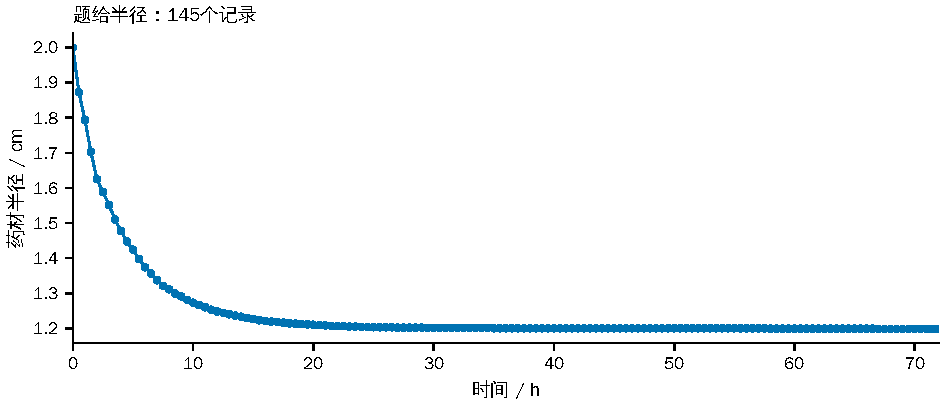
\includegraphics[width=\linewidth]{figures/raw_q4_radius.pdf}
\caption{几何输入：附件2全部145条半径记录及分段线性重建，保留平台段，不向72小时外延拓。}\label{fig:q4-radius}
\end{figure}

收缩后，同一个物理半径位置可能先在药材内，随后离开计算域。输出位置$r$只有在$r\leq R(t)$时才有温度或含水率意义。域外值不等于零，也不是随机缺测，而是该时刻没有药材。问题四工作簿因此保留0至1.9厘米的固定位置列，额外设置随$R(t)$变化的真实表面列。域外单元格为空；论文表格用破折号表示相同含义。早期1.5厘米处仍可能有值，只有题目表6从6小时开始的各行，该位置才全部在药材外。

问题一工作簿输出1至1800秒。问题二的温度、水分浓度两工作表均从1秒输出至问题三的严格整秒终点206902秒，时间间隔1秒，半径位置为0、0.1、\ldots、2.0厘米；每表有206902个时间行。题目表3、表4在论文中仍只列0.5至3.0小时。问题二全过程逐秒文件与问题三逐分钟文件是同一初边值解的两种输出分辨率，不相互替代。问题三、四每60秒输出一次，并补入不重复的严格整秒终点，保证最后一行与终止判据一致。

\section{模型假设、物性与热湿耦合方程}
\subsection{状态、符号及必要闭合}
记$\theta(r,t)$为摄氏温度，$C(r,t)$为干基含水率，$R(t)$为外半径，$\rho_h$为仅参与有效热容量的经验参数，$c_p$、$k$、$D$分别为题设比热、导热率和水分扩散系数。另用$\rho_d$表示质量守恒中的单位当前体积干物质质量，二者不混用。绝对温度仅在Arrhenius指数中使用，定义为$T_K=\theta+273.15$。表\ref{tab:symbol}集中列出单位，避免把传热系数$h$与时间小时混同，或把以米每秒计的传质系数直接当成质量通量。

\begin{table}[htbp]\centering\small
\caption{主要符号与量纲}\label{tab:symbol}
\begin{tabular}{lll}
\toprule
符号 & 含义 & 单位\\
\midrule
$\theta,\theta_\infty$ & 药材温度、环境温度 & 摄氏度\\
$C,C_e$ & 干基含水率、有效平衡含水率 & kg/kg\\
$r,R,x=r/R$ & 物理半径、外半径、归一化半径 & m、m、1\\
$\rho_h,c_p$ & 热容量经验参数、比热 & kg/m$^3$、J/(kg K)\\
$\rho_d$ & 单位当前体积干物质质量 & kg/m$^3$\\
$k,D$ & 导热率、水分扩散系数 & W/(m K)、m$^2$/s\\
$h,h_m$ & 表面对流换热、有效传质系数 & W/(m$^2$ K)、m/s\\
$A=\rho_h c_p$ & 有效体积热容量 & J/(m$^3$ K)\\
$t_*,t_{\rm int}$ & 越阈事件、严格整秒终点 & s\\
$\overline C,C_{\max}$ & 径向体积权均值、全域最大值 & kg/kg\\
\bottomrule
\end{tabular}
\end{table}

本文建立理想化、有效参数的一维径向传热传质模型，目标是在题给数据和约定条件下描述变化规律，而非还原特定药材的完整真实物理过程。表\ref{tab:closure}集中给出模型闭合；后续推导、检验和对照均保持这些定义，不另行改变模型族。

\begin{table}[htbp]\centering\small
\caption{模型闭合与各项约定承担的作用}\label{tab:closure}
\begin{tabularx}{\linewidth}{lXX}
\toprule
对象 & 明确约定 & 在模型中的作用\\
\midrule
空间与几何 & 轴向、周向均匀，径向可非均匀；长度不变 & 只求径向场；“全域”限于该场\\
外部水分 & $C_e=W_a$为有效边界定义 & 将附件记录用于Robin传质驱动力，不识别真实吸附平衡\\
能量 & 忽略蒸发潜热，无内部热源 & 采用$A(C)\theta_t$的有效热容量闭合\\
两类密度 & $\rho_h$只用于$A=\rho_h c_p$；$\rho_d$用于干质量守恒 & 不附加$\rho_h=(1+C)\rho_d$关系\\
未观测工况 & $t>4$小时取50摄氏度、0.05 kg/kg & 定义长期边界；以情景扰动评估其影响\\
问题四运动 & 同调径向收缩，$x=r/R(t)$为材料坐标 & 外半径轨迹确定内部速度$v=r\dot R/R$\\
干固体 & 初始密度空间均匀、干质量不流失 & 得到$\rho_d(t)R(t)^2=\rho_{d0}R_0^2$\\
\bottomrule
\end{tabularx}
\end{table}

其中同调性并非由外轮廓数据反演所得，而是使移动域方程闭合的运动定义。忽略潜热也不意味着题给经验参数已经吸收了该机制。热、质传递系数分别取题给$h=25$ W/(m$^2$ K)和$h_m=8\times10^{-7}$ m/s，四问均保持不变。

\subsection{固定半径下的控制方程}
对于问题一至三，$0\leq r\leq R_0$、$R_0=0.02$米。采用式\eqref{eq:pdes}给出局部热湿传递，题设变系数保留在散度内部。若直接写成$k$乘拉普拉斯算子，会遗漏导热率梯度的作用；若把$1/(\rho_h c_p)$也放进散度，则改变了原来的热容量模型。两种误写在常系数时可能看不出来，在问题二至四中会影响温湿反馈。

\begin{equation}\label{eq:pdes}
\begin{aligned}
A(C)\frac{\partial\theta}{\partial t}
&=\frac1r\frac{\partial}{\partial r}
       \left(rk(C)\frac{\partial\theta}{\partial r}\right),\\
\frac{\partial C}{\partial t}
&=\frac1r\frac{\partial}{\partial r}
       \left(rD(\theta,C)\frac{\partial C}{\partial r}\right).
\end{aligned}
\end{equation}

初始条件见式\eqref{eq:initial}。温度初始与空气温度相同，初始热通量为零；含水率初始显著高于有效平衡值，表面在开始时立即向外传质。均匀初值的零径向梯度与初始Robin水分通量存在角点不相容，这是扩散初边值问题常见的短时边界层，不应通过修改初始表面含水率来消除。隐式积分从均匀初态发展该边界层，早期网格和步长检查因而不可省略。

\begin{equation}\label{eq:initial}
\theta(r,0)=28,\qquad C(r,0)=2.55,\qquad 0\leq r\leq R_0.
\end{equation}

中心满足轴对称条件，表面采用有限交换阻力的Robin条件，见式\eqref{eq:bc}。符号按外法向为正定义：脱水时$C_s>C_e$，向外水分通量为正；升温时$\theta_s<\theta_\infty$，向外热通量为负。这一符号约定使两类边界共享同一通量实现，减少在热量进入、质量流出之间分别判断符号的风险。

\begin{equation}\label{eq:bc}
\begin{aligned}
\theta_r(0,t)&=0,\qquad C_r(0,t)=0,\\
-k_s\theta_r(R_0,t)&=h(\theta_s-\theta_\infty),\qquad h=25,\\
-D_sC_r(R_0,t)&=h_m(C_s-C_e),\qquad h_m=8\times10^{-7}.
\end{aligned}
\end{equation}

式\eqref{eq:pdes}中的$A(C)\theta_t$不能替换为$\partial_t[A(C)\theta]$，后者多出$\theta A'(C)C_t$，会改变表\ref{tab:closure}定义的能量方程。本文因此检查通量离散与该有效方程的一致性，并对干基水分单独建立守恒关系，不把它扩展为未定义的多相总焓验证。

\subsection{三组题设物性}
问题一采用式\eqref{eq:props1}。虽然热方程为常系数线性扩散，水分方程仍是非线性的：随着表面干燥，$D$会减小，局部扩散阻力逐渐增加。因此问题一也不能使用一个常数扩散系数替代整个水分过程。

\begin{equation}\label{eq:props1}
\rho_h=820,\quad c_p=2600,\quad k=0.36,\quad
D=7\times10^{-9}\exp(-0.89/C).
\end{equation}

问题二、三共享式\eqref{eq:props23}，其中指数温度必须使用开尔文。水分降低使有效热容量和导热率变化，温度升高则通过指数项促进水分扩散。这种双向作用要求在每一次隐式迭代中依据当前状态更新物性，不能仅在整秒输出时更新。问题二从$t=0$即使用本组物性，不是在问题一半小时末状态上切换。

\begin{equation}\label{eq:props23}
\begin{aligned}
\rho_h&=650+128C,&
c_p&=1450+\frac{2736C}{1+C},\\
k&=0.21+\frac{0.38C}{1+C},&
D&=0.0024\exp\left(-\frac{0.45}{C}-\frac{3850}{T_K}\right).
\end{aligned}
\end{equation}

问题四使用式\eqref{eq:props4}，并同时引入实测半径。它不是仅把问题三的$R_0$换成$R(t)$，因为所有有效物性函数也发生变化。后文设置保持式\eqref{eq:props4}而固定半径的反事实，以区分几何与物性的作用。

\begin{equation}\label{eq:props4}
\begin{aligned}
\rho_h&=760+90C,&
c_p&=1850+\frac{2150C}{1+C},\\
k&=0.12+\frac{0.20C}{1+C},&
D&=0.00042\exp\left(-\frac{0.30}{C}-\frac{3850}{T_K}\right).
\end{aligned}
\end{equation}

图\ref{fig:q3-dfunction}只展示式\eqref{eq:props23}在28和50摄氏度下的函数值，不是新增材料测量。高水分区扩散系数变化较缓，接近有效边界低含水率时则跨越多个数量级。这说明干燥后期可能由低水分表层形成的高阻力控制，而非保持初始扩散速度。与柱状食品热湿耦合研究中的温度依赖处理相一致\cite{tzempelikos2015quince}，本文保留Arrhenius结构；文献在此仅说明方法背景，不作为题给物性或一维假设的实验证据。

\begin{figure}[htbp]\centering
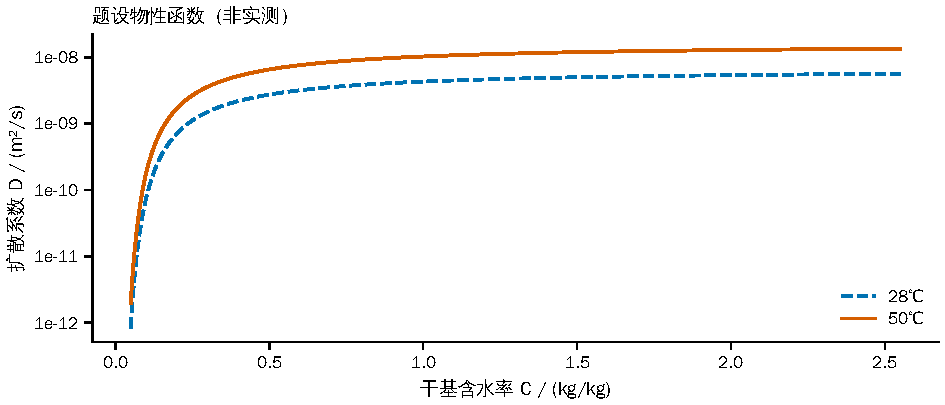
\includegraphics[width=\linewidth]{figures/raw_q3_diffusivity.pdf}
\caption{问题二、三的题设扩散函数：28与50摄氏度下，低含水率区的$D$迅速下降；纵轴为对数刻度，非实验数据。}\label{fig:q3-dfunction}
\end{figure}

\section{守恒有限体积与隐式求解}
\subsection{表面加密网格及控制体}
令$x=r/R$，固定域时$R=R_0$。使用包含中心和表面的$N+1$个节点，按式\eqref{eq:grid}向表面加密。这里$N$是区间数，不是节点数；近表面的较密节点用于分辨后期含水率陡降区域。网格分配只说明分辨率放在哪里，精度是否足够仍由多网格比较确定，本文不据此宣称相对均匀网格的等精度计算效率优势。

\begin{equation}\label{eq:grid}
x_i=1-\left(1-\frac{i}{N}\right)^2,\quad i=0,\ldots,N;\qquad
x_{i+1/2}=\frac{x_i+x_{i+1}}2,\quad
w_i=\frac{x_{i+1/2}^2-x_{i-1/2}^2}{2}.
\end{equation}

两端面分别取$x_{-1/2}=0$和$x_{N+1/2}=1$。$w_i$来自柱坐标体积权重$\int x\,dx$，而不是简单的节点间距；因此靠外的环形控制体与中心控制体具有不同权重。全部权重之和为$1/2$，径向平均可以直接计算为$2\sum_iw_iC_i$。若把这些节点当成等体积样本求算术平均，会偏置截面平均含水率。

对一般变量$u$、扩散系数$a$，在相邻节点之间使用调和平均$a_{i+1/2}$，构造式\eqref{eq:flux}的向内通量记号$G$。两个半段串联的扩散阻力对应调和平均，尤其有利于保留低扩散系数表层的阻滞作用。这里的$G$包含径向面权重，但尚未除以控制体和$R^2$；它不是以千克每秒计的实际出水速率。

\begin{equation}\label{eq:flux}
\begin{aligned}
a_{i+1/2}&=\frac{2a_i a_{i+1}}{a_i+a_{i+1}},\\
G_{i+1/2}&=x_{i+1/2}a_{i+1/2}
               \frac{u_{i+1}-u_i}{x_{i+1}-x_i},\\
G_{-1/2}&=0,\qquad
G_{N+1/2}=R\beta(u_\infty-u_N).
\end{aligned}
\end{equation}

温度取$(u,a,\beta,u_\infty)=(\theta,k,h,\theta_\infty)$，水分取$(C,D,h_m,C_e)$。于是半离散方程统一为式\eqref{eq:fvm}，其中温度方程的$q_i=A_i$，水分方程的$q_i=1$。相邻控制体使用同一个面通量且符号相反，内部通量在全域求和时精确相消，这是归一化水分平衡的基础。

\begin{equation}\label{eq:fvm}
\frac{du_i}{dt}=
\frac{G_{i+1/2}-G_{i-1/2}}{R^2w_iq_i}.
\end{equation}

中心的$1/r$表观奇点不通过人为加一个小半径回避，而由中心控制体积分自然消除。由$x_{1/2}=x_1/2$可得中心极限离散为式\eqref{eq:center}，系数为4而不是平板几何的2。这个差异若写错，会影响中心升温与最终中心脱水时间，却未必在表面曲线上明显暴露。

\begin{equation}\label{eq:center}
\frac{du_0}{dt}=
\frac{4a_{1/2}(u_1-u_0)}{R^2x_1^2q_0}.
\end{equation}

\subsection{刚性积分与解析雅可比}
加密网格使最小空间尺度变小，而低含水率又使不同位置的扩散时间相差很大，半离散系统具有刚性。本文使用BDF隐式积分，并提供解析稀疏雅可比。状态向量同时包含全部温度、水分以及用于平衡检查的累计归一化损失；各节点只与相邻节点直接耦合，雅可比具有稀疏块结构。热湿交叉块不能忽略：$C$改变热容量与导热率，$\theta$改变水分扩散系数。

以调和平均$H(a,b)=2ab/(a+b)$为例，其导数及问题二、三的$D$导数见式\eqref{eq:jacderiv}。温度方程还必须包含热容量分母求导产生的修正$-\dot\theta_i A'_i/A_i$。若只对导热通量求导，得到的不是完整雅可比，可能降低长时稳态附近的求解稳定性。解析形式同时避免靠数值差分估计极小导数时产生不必要的运行警告。

\begin{equation}\label{eq:jacderiv}
\begin{aligned}
\frac{\partial H}{\partial a}&=\frac{2b^2}{(a+b)^2},&
\frac{\partial H}{\partial b}&=\frac{2a^2}{(a+b)^2},\\
\frac{\partial D}{\partial\theta}&=D\frac{3850}{T_K^2},&
\frac{\partial D}{\partial C}&=D\frac{0.45}{C^2}.
\end{aligned}
\end{equation}

名义相对容差取$10^{-8}$，温度绝对容差$10^{-8}$摄氏度，含水率及累计损失绝对容差$10^{-10}$。前四小时最大时间步为15秒，之后为600秒；步长由隐式误差估计自动控制，最大值不是实际固定步长。四小时处分段处理环境延拓。半径曲线虽然在采样点改变斜率，但在随体方程中仅以连续的$R(t)$进入，求解器不需要用不稳定的数值差分估计半径导数。

输出时间与内部积分步不同。程序利用每一积分段的连续输出，在题目指定时刻采样，再用保形分段三次插值映射到指定物理半径。对于单调的径向含水率剖面，保形插值不产生超出端点的新极值。输出四位小数只发生在Excel和论文展示阶段，误差比较、阈值判定及均值积分始终使用未舍入浮点状态。读取跨越分段边界或顺序不规则的请求时刻时，程序逐段分配并检查每个时刻均被覆盖，避免遗漏或读取未初始化状态。

\section{问题一：常热物性下的短时温湿分布}
\subsection{指定位置与时刻的计算结果}
表\ref{tab:paper1}和表\ref{tab:paper2}列出100、300、600、900、1200、1500、1800秒时，半径0、0.5、1.0、1.5、2.0厘米处的温度与干基含水率。结果由最终640区间网格的未舍入数值解采样得到，完整逐秒数据保存在工作簿1中。

\input{tables/table1.tex}
\begin{table}[htbp]
\centering\small
\caption{问题一指定时刻的干基含水率（对应题目表2，单位：kg/kg）}\label{tab:paper2}
\begin{tabular}{rrrrrr}
\toprule
时间/s & 0 cm & 0.5 cm & 1.0 cm & 1.5 cm & 2.0 cm \\
\midrule
100 & 2.5500 & 2.5500 & 2.5500 & 2.5500 & 2.2470 \\
300 & 2.5500 & 2.5500 & 2.5500 & 2.5492 & 2.0508 \\
600 & 2.5500 & 2.5500 & 2.5500 & 2.5353 & 1.8770 \\
900 & 2.5500 & 2.5500 & 2.5497 & 2.5045 & 1.7547 \\
1200 & 2.5500 & 2.5500 & 2.5482 & 2.4646 & 1.6586 \\
1500 & 2.5500 & 2.5499 & 2.5445 & 2.4206 & 1.5787 \\
1800 & 2.5500 & 2.5497 & 2.5383 & 2.3755 & 1.5102 \\
\bottomrule
\end{tabular}
\end{table}



0.50小时，中心和表面温度分别为33.5753、36.7856摄氏度，相差3.2102摄氏度；中心含水率为2.5500，接近初值，表面已降至1.5102。热量已影响整个截面，明显失水主要发生在近表面区域。

图\ref{fig:q1-profiles}给出100、600和1800秒的径向剖面。温度在中心附近平坦，向表面升高；含水率则在表面最低，向中心逐渐接近初值。两组剖面反映了热量传入与水分排出的不同进程。

\begin{figure}[htbp]\centering
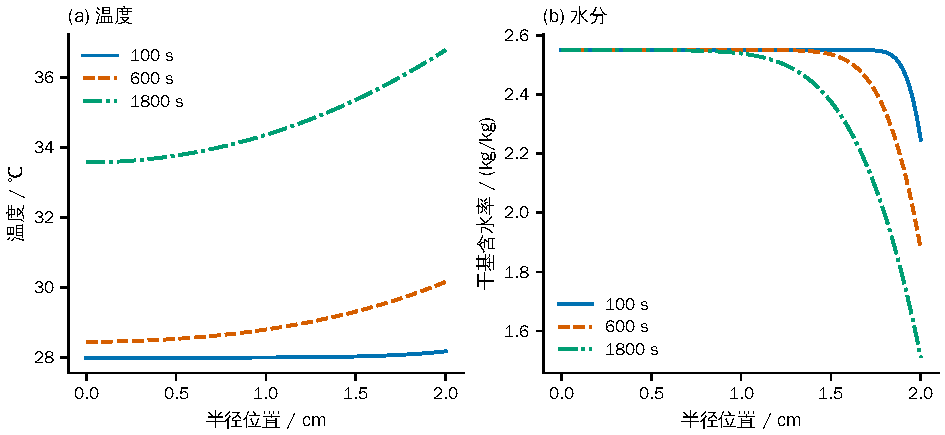
\includegraphics[width=\linewidth]{figures/result_q1_profiles.pdf}
\caption{问题一在100、600和1800秒的径向温湿剖面，同一时刻采用相同颜色与线型。}\label{fig:q1-profiles}
\end{figure}

\subsection{传递尺度及边界阻力解释}
问题一的热扩散率为$k/(\rho_h c_p)=1.6886\times10^{-7}$平方米每秒，初始水分扩散系数为$4.9377\times10^{-9}$平方米每秒，前者约为后者的34倍。在相同几何尺度下，热量比水分更快影响内部。以半径定义式\eqref{eq:bi}中的Biot数，热Biot数为1.3889，需保留内部温度梯度。

\begin{equation}\label{eq:bi}
\alpha=\frac{k}{\rho_h c_p},\qquad
{\rm Bi}_T=\frac{hR}{k},\qquad
{\rm Bi}_C=\frac{h_mR}{D}.
\end{equation}

初始水分Biot数约为3.2404。将$C=0.15$代入题设函数，得到$D=1.8547\times10^{-11}$平方米每秒，相应水分Biot数约为862.65。这里用函数值说明低含水率时内部阻力的增大，所取$C=0.15$并非问题一在0.50小时的实际状态。计算中仍按各节点状态更新$D$。

表面含水率在短时间内下降较快，表面状态与环境之间仍保留有限差值。Robin条件通过题给传递系数确定交换速率，描述表面温度和含水率对环境变化的响应。

\section{问题二：变物性热湿耦合过程}
\subsection{前三小时的结果与反馈}
问题二的六个指定时刻结果见表\ref{tab:paper3}和表\ref{tab:paper4}。0.50小时，中心、表面温度分别为32.1892、35.4130摄氏度，均低于问题一；表面含水率为1.6486，高于问题一的1.5102。这一差异来自热容量、导热率和扩散函数的共同改变，传热及传质系数保持不变。

\begin{table}[htbp]
\centering\small
\caption{问题二指定时刻的温度（对应题目表3，单位：摄氏度）}\label{tab:paper3}
\begin{tabular}{rrrrrr}
\toprule
时间/h & 0 cm & 0.5 cm & 1.0 cm & 1.5 cm & 2.0 cm \\
\midrule
0.5000 & 32.1892 & 32.3821 & 32.9659 & 33.9608 & 35.4130 \\
1 & 40.3816 & 40.5536 & 41.0605 & 41.8782 & 42.9976 \\
1.5000 & 45.8468 & 45.9348 & 46.1930 & 46.6051 & 47.1401 \\
2 & 48.4502 & 48.4881 & 48.5984 & 48.7736 & 49.0033 \\
2.5000 & 49.4670 & 49.4792 & 49.5136 & 49.5653 & 49.6609 \\
3 & 49.8495 & 49.8553 & 49.8746 & 49.9101 & 49.9664 \\
\bottomrule
\end{tabular}
\end{table}


\begin{table}[htbp]
\centering\small
\caption{问题二指定时刻的干基含水率（对应题目表4，单位：kg/kg）}\label{tab:paper4}
\begin{tabular}{rrrrrr}
\toprule
时间/h & 0~cm & 0.5~cm & 1.0~cm & 1.5~cm & 2.0~cm \\
\midrule
0.5000 & 2.5499 & 2.5489 & 2.5256 & 2.3257 & 1.6486 \\
1.0000 & 2.5257 & 2.4948 & 2.3578 & 2.0230 & 1.4711 \\
1.5000 & 2.3861 & 2.3256 & 2.1344 & 1.8020 & 1.3476 \\
2.0000 & 2.1709 & 2.1084 & 1.9236 & 1.6259 & 1.2311 \\
2.5000 & 1.9566 & 1.9006 & 1.7360 & 1.4720 & 1.1166 \\
3.0000 & 1.7662 & 1.7165 & 1.5702 & 1.3333 & 1.0081 \\
\bottomrule
\end{tabular}
\end{table}


3小时，中心、表面温度分别为49.8495、49.9664摄氏度，径向温差为0.1169摄氏度；含水率分别为1.7662、1.0081，相差0.7581。温度已接近均匀，水分仍有明显梯度。

图\ref{fig:q2-fields}在共同的时间与半径坐标上展示前三小时温湿场。温度由外向内升高，含水率由表面向内降低。升温逐渐接近完成时，水分迁移仍在继续，后续烘干主要受内部扩散及表层阻力影响。

\begin{figure}[htbp]\centering
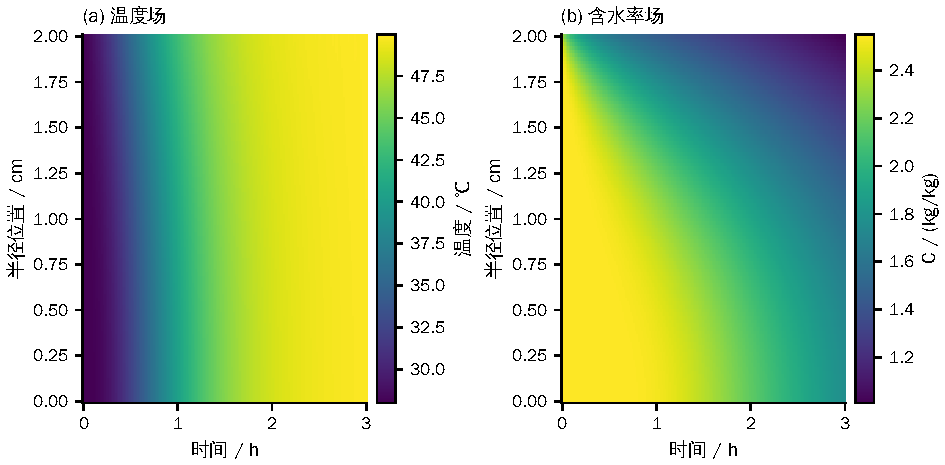
\includegraphics[width=\linewidth]{figures/result_q2_fields.pdf}
\caption{问题二前三小时的温度与含水率场，按60秒间隔和101个径向重建点展示。}\label{fig:q2-fields}
\end{figure}

\subsection{扩散函数沿计算轨迹的变化}
扩散系数随温度升高而增大，随含水率降低而减小。图\ref{fig:q2-dtrajectory}将求得的温湿场代入题设函数，展示两种作用共同形成的局部扩散系数变化，色标采用对数形式。

\begin{figure}[htbp]\centering
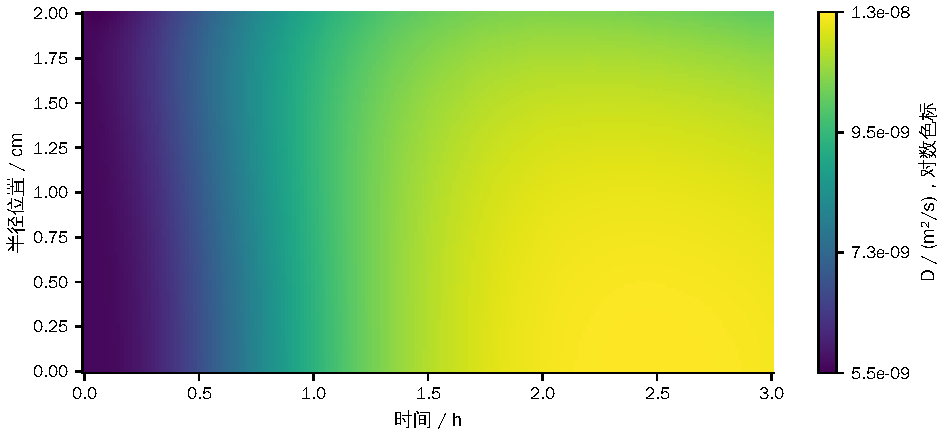
\includegraphics[width=\linewidth]{figures/process_q2_diffusion.pdf}
\caption{问题二前三小时的局部扩散系数，由温湿解代入题设函数得到，色标采用对数形式。}\label{fig:q2-dtrajectory}
\end{figure}

在50摄氏度下，$C=2.55$时的扩散系数约为$1.3471\times10^{-8}$平方米每秒；$C=0.15$时为$8.0012\times10^{-10}$，$C=0.05$时降至$1.9833\times10^{-12}$。即使表层已升温，含水率降低仍可使其成为低扩散区，这有助于解释后期脱水减慢。

含水率降低时，有效体积热容量和导热率均下降。前者使同等净热流引起的温度变化加快，后者减小内部导热能力；两种作用由联立方程共同确定。问题三延续该初边值问题，计算至全域含水率阈值。

问题二、三采用同一积分解。问题二从连续解中逐秒采样，问题三按60秒间隔输出，并由事件函数确定终点。两者的区别在于结果呈现方式。

\section{问题三：固定半径的全域达标时间}
\subsection{事件判据与三种含水指标}
“药材内部各处均低于0.15”对应最大值条件。式\eqref{eq:metrics}分别定义径向最大含水率、体积权均值和表面含水率。计算在全部节点上取最大值，保形径向重建保持节点间的单调性。在已检查时刻，最大值位于中心附近；终点算法仍使用全部节点的最大值。

\begin{equation}\label{eq:metrics}
C_{\max}(t)=\max_{0\leq r\leq R(t)}C(r,t),\qquad
\overline C(t)=\frac{2}{R(t)^2}\int_0^{R(t)}rC(r,t)\,dr,\qquad
C_s(t)=C(R(t),t).
\end{equation}

先定位$C_{\max}-0.15$由正到负的事件，再按式\eqref{eq:event}确定严格小于阈值的整秒输出时刻。由于题目采用严格不等式，事件恰在整数秒发生时仍取下一秒，并用未舍入的全部节点状态检查该时刻。

\begin{equation}\label{eq:event}
C_{\max}(t_*)=0.15\ \text{且向下穿越},\qquad
t_{\rm int}=\lfloor t_*\rfloor+1,\qquad
C_{\max}(t_{\rm int})<0.15.
\end{equation}

图\ref{fig:q3-threshold}比较三种含水指标。按60秒保存轨迹线性插值，表面值约在12.5521小时达到0.15，均值约在36.0251小时达到0.15；最大值的事件时间为57.4728小时。前两个时间是轨迹插值近似值，最大值时间由事件求根得到。采用最大值判据能覆盖内部较慢脱水的位置。

\begin{figure}[htbp]\centering
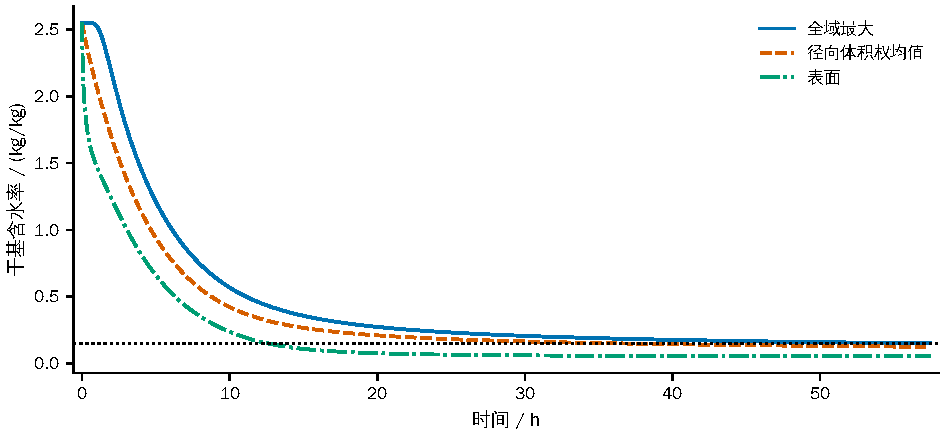
\includegraphics[width=\linewidth]{figures/process_q3_threshold.pdf}
\caption{问题三的最大、平均及表面含水率，按60秒间隔并补入终点；点线表示阈值0.15。}\label{fig:q3-threshold}
\end{figure}

\subsection{终点数值及每六小时结果}
最终网格下，问题三的越阈时间为57.4728小时。终点表面含水率约为0.0527，体积权均值约为0.1243。表\ref{tab:paper5}列出每6小时及严格终点的指定位置结果。

\begin{table}[htbp]
\centering\small
\caption{问题三每6 h及严格终点的干基含水率（对应题目表5）}\label{tab:paper5}
\begin{tabular}{rrrrrr}
\toprule
时间/h & 0~cm & 0.5~cm & 1.0~cm & 1.5~cm & 2.0~cm \\
\midrule
6 & 1.0170 & 0.9881 & 0.9015 & 0.7550 & 0.5328 \\
12 & 0.4561 & 0.4432 & 0.4031 & 0.3297 & 0.1642 \\
18 & 0.2988 & 0.2915 & 0.2687 & 0.2253 & 0.0845 \\
24 & 0.2378 & 0.2327 & 0.2167 & 0.1855 & 0.0665 \\
30 & 0.2058 & 0.2018 & 0.1892 & 0.1641 & 0.0598 \\
36 & 0.1859 & 0.1825 & 0.1718 & 0.1504 & 0.0566 \\
42 & 0.1721 & 0.1691 & 0.1597 & 0.1407 & 0.0549 \\
48 & 0.1618 & 0.1592 & 0.1507 & 0.1334 & 0.0537 \\
54 & 0.1539 & 0.1514 & 0.1436 & 0.1277 & 0.0530 \\
57.4728 & 0.1500 & 0.1477 & 0.1402 & 0.1249 & 0.0527 \\
\bottomrule
\end{tabular}
\par\smallskip\begin{minipage}{0.93\linewidth}\footnotesize 数值单位为 kg/kg。末行使用严格整秒终点，时间转为小时后显示四位小数；中心显示 0.1500 是舍入结果，严格不等式按未舍入值检查。\end{minipage}
\end{table}


表\ref{tab:paper5}显示，中心含水率由6小时的1.0170降至12小时的0.4561，48小时仍为0.1618，54小时为0.1539。接近阈值时，绝对剩余差值虽小，仍需较长时间继续脱水。这与低含水率区扩散系数迅速下降的特征一致。

图\ref{fig:q3-terminal}给出终点径向剖面。中心附近接近阈值，表面接近且略高于有效边界值0.05。表面与环境间的正含水率差维持向外传质，使内部水分继续排出。

\begin{figure}[htbp]\centering
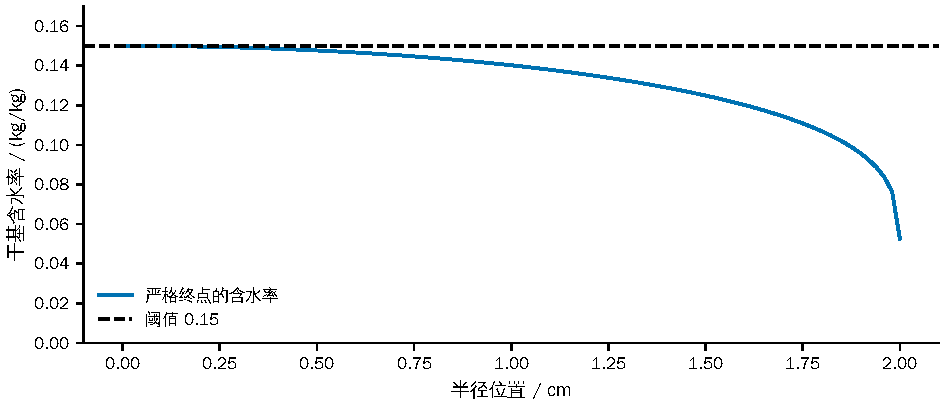
\includegraphics[width=\linewidth]{figures/result_q3_terminal.pdf}
\caption{问题三终点的径向含水率分布，中心接近阈值，表面含水率较低。}\label{fig:q3-terminal}
\end{figure}

\section{问题四：实测收缩下的移动边界}
\subsection{随体坐标与运动项}
在均匀径向收缩假设下，材料速度为$v(r,t)=r\dot R/R$。令$x=r/R(t)$，对随材料输运的标量$u$定义$U(x,t)=u(R(t)x,t)$，可得式\eqref{eq:ale}。固定空间时间导数中的坐标变化项与材料平流项抵消，随体坐标下的时间导数即为物质导数。

\begin{equation}\label{eq:ale}
\left.\frac{\partial u}{\partial t}\right|_r
=\left.\frac{\partial U}{\partial t}\right|_x
-\frac{x\dot R}{R}U_x,\qquad
v\,u_r=\frac{x\dot R}{R}U_x,\qquad
\frac{{\rm D}u}{{\rm D}t}=U_t.
\end{equation}

移动边界干燥中可用ALE方法描述网格和材料运动\cite{seyedabadi2017ale}。这里采用网格随材料均匀收缩的情形，固定$x$对应同一材料位置。

随体坐标下的方程和表面条件见式\eqref{eq:moving}，其中时间导数均在固定$x$下计算。沿用有限体积离散，在各时刻更新半径和问题四物性。内部扩散含$R(t)^{-2}$因子，归一化表面交换含$R(t)^{-1}$因子，二者共同决定收缩后的传递速度。

\begin{equation}\label{eq:moving}
\begin{aligned}
A(C)\theta_t&=\frac{1}{R(t)^2x}
                \partial_x\!\left(xk(C)\theta_x\right),\\
C_t&=\frac{1}{R(t)^2x}
                \partial_x\!\left(xD(\theta,C)C_x\right),\\
-k_s\theta_x(1,t)&=R(t)h(\theta_s-\theta_\infty),\\
-D_sC_x(1,t)&=R(t)h_m(C_s-C_e).
\end{aligned}
\end{equation}

\subsection{干基变量为何不直接增加压缩项}
干基含水率为水质量与干物质质量之比。均匀收缩使单位体积内两种质量同时变化，压缩本身保持该比值。设干固体密度$\rho_d(t)$在截面上均匀，长度不变且干质量守恒，则$\rho_dR^2$为常数。取相对干固体的扩散通量为$-\rho_dD\nabla C$，由水分与干固体连续性方程得到式\eqref{eq:drybasis}。

\begin{equation}\label{eq:drybasis}
\begin{aligned}
\frac{{\rm D}\rho_d}{{\rm D}t}+\rho_d\nabla\!\cdot v&=0,\\
\rho_d\frac{{\rm D}C}{{\rm D}t}
&=\nabla\!\cdot(\rho_dD\nabla C),\\
\rho_d(t)=\rho_{d0}\left(\frac{R_0}{R(t)}\right)^2\quad&\Longrightarrow\quad
\frac{{\rm D}C}{{\rm D}t}=\nabla\!\cdot(D\nabla C).
\end{aligned}
\end{equation}

空间均匀的$\rho_d(t)$可从散度中提出并约去，得到式\eqref{eq:moving}中的水分方程，无需附加$-C\nabla\!\cdot v$项。初始密度$\rho_{d0}>0$也在归一化方程中约去，计算无需另赋数值。若改用单位当前体积的水浓度，压缩项的形式将随变量定义改变；相关移动边界研究采用过这类体积变量\cite{adrover2020pears}。

题给$\rho_h=760+90C$按表\ref{tab:closure}用于有效热容量，水分收支则相对于不变干质量归一化。两种参数分别承担能量闭合和质量守恒的作用。

\subsection{含水率场、域外位置与严格终点}
图\ref{fig:q4-moving}以物理半径为纵轴，黑线表示插值半径$R(t)$，域外留白。固定物理半径对应水平线，而同一材料点随$r=xR(t)$运动，应沿该轨迹读取其状态变化。

\begin{figure}[htbp]\centering
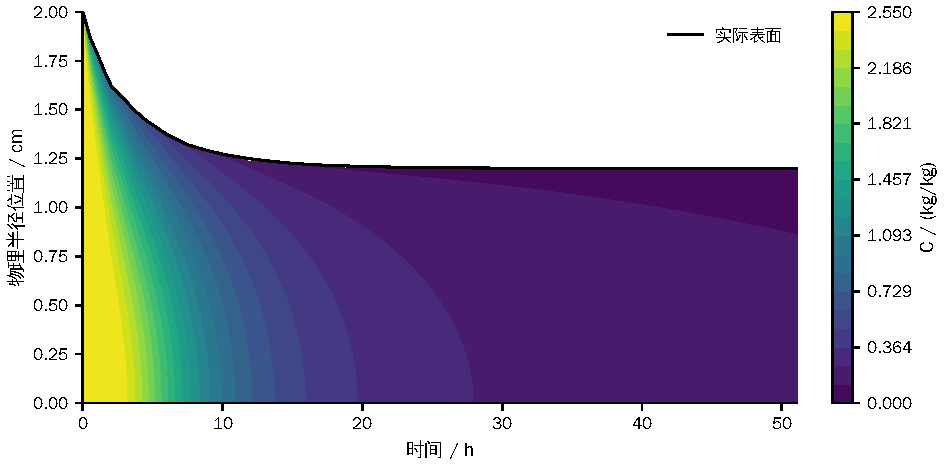
\includegraphics[width=\linewidth]{figures/process_q4_moving.pdf}
\caption{问题四的移动域含水率场，按60秒间隔并补入终点；黑线为当前表面，域外留白。}\label{fig:q4-moving}
\end{figure}

采用与问题三相同的最大含水率判据，问题四的越阈时间为51.0908小时。终点表面含水率约为0.0526，体积权均值约为0.1184，半径为1.2000厘米。终点位于半径记录的72小时范围内。

表\ref{tab:paper6}列出每6小时及严格终点的指定位置含水率。在这些表列时刻，0、0.5、1.0厘米均位于药材内，1.5厘米均在域外。表面列对应实际$R(t)$处状态，随半径轨迹变化。工作簿4中的20099个域外位置按定义留空。

\begin{table}[htbp]
\centering\small
\caption{问题四每6小时及严格终点的干基含水率（对应题目表6）}\label{tab:paper6}
\begin{tabular}{rrrrrr}
\toprule
时间/h & 0 cm & 0.5 cm & 1.0 cm & 1.5 cm & 移动表面 \\
\midrule
6 & 1.7196 & 1.5377 & 1.0226 & --- & 0.4207 \\
12 & 0.7377 & 0.6546 & 0.4083 & --- & 0.1670 \\
18 & 0.4087 & 0.3686 & 0.2397 & --- & 0.0892 \\
24 & 0.2851 & 0.2611 & 0.1790 & --- & 0.0673 \\
30 & 0.2263 & 0.2094 & 0.1493 & --- & 0.0595 \\
36 & 0.1928 & 0.1797 & 0.1317 & --- & 0.0560 \\
42 & 0.1712 & 0.1604 & 0.1200 & --- & 0.0541 \\
48 & 0.1561 & 0.1468 & 0.1116 & --- & 0.0530 \\
51.0908 & 0.1500 & 0.1413 & 0.1081 & --- & 0.0526 \\
\bottomrule
\end{tabular}
\par\smallskip\begin{minipage}{0.93\linewidth}\footnotesize “---”表示该时刻位置已在药材外，结果工作簿对应单元格为空；数值单位为 kg/kg。末行使用严格整秒终点，时间转为小时后显示四位小数；中心显示 0.1500 是舍入结果，严格不等式按未舍入值检查。\end{minipage}
\end{table}



问题四在6小时的中心含水率为1.7196，高于问题三的1.0170；42小时为0.1712，略低于问题三的0.1721。按60秒最大含水率轨迹插值，两曲线约在41.2小时交叉。物性变化与扩散距离缩短共同影响全过程，问题四在早期较湿，最终却较早达到阈值。

\section{数值验证与误差分析}
数值验证围绕三个问题展开：离散格式是否正确，空间与时间分辨率是否足够，以及终点结果是否稳定。表\ref{tab:verification-map}列出各项检验的参照对象与作用。

\begin{table}[htbp]\centering\small
\caption{验证项目、参照对象与可识别的错误}\label{tab:verification-map}
\begin{tabularx}{\linewidth}{lXX}
\toprule
检验 & 参照对象 & 主要识别问题\\
\midrule
固定域解析模态 & Robin边界Bessel解与精确越阈时间 & 柱坐标算子、中心和表面符号、事件定位\\
移动域非均匀模态 & 变半径零通量解析解 & 几何因子是否真正随时间更新\\
几何因子对照算例 & 只把$R(t)^{-2}$冻结为$R_0^{-2}$ & 固定几何因子对求解误差的影响\\
水分收支 & 离散均值与累计边界损失 & 面通量、积分权重和干基归一化\\
雅可比方向差分 & 实际右端的中心差分 & 状态及交叉导数是否一致\\
网格与容差复验 & 同一工况下更细离散结果 & 本题场与终点对数值设置的敏感性\\
\bottomrule
\end{tabularx}
\end{table}

\subsection{解析极限、封闭场与导数检查}
对常扩散系数$d_0=10^{-5}$平方米每秒、半径0.02米、$C_e=0.05$、$h_m=d_0/R$的算例，取式\eqref{eq:bessel}的Bessel模态初值。其中$\beta$为$\beta J_1(\beta)=J_0(\beta)$的第一正根，解析解同时满足中心对称和Robin表面条件。该组参数专用于数值验证。

\begin{equation}\label{eq:bessel}
C(r,t)=0.05+0.20J_0\left(\beta\frac rR\right)
       \exp\left(-\frac{d_0\beta^2}{R^2}t\right),\qquad
t_{\rm exact}=\frac{R^2\log2}{d_0\beta^2}.
\end{equation}

采用160个区间时，精确越阈时间为17.581493358秒，数值事件时间为17.581482896秒，相差约$1.05\times10^{-5}$秒。该算例共同检验柱坐标离散、中心处理、表面通量符号和事件定位。另取零传质系数与均匀初值，离散右端为零，封闭均匀场保持不变。

以方向差分比较$J(y)p$和$[F(y+\varepsilon p)-F(y-\varepsilon p)]/(2\varepsilon)$，检查解析雅可比与方程右端的一致性。检验覆盖四问，并在常湿、低湿、均匀及加密网格下比较16组块导数，最大相对差约为$3.78\times10^{-10}$。

\subsection{非均匀初值的移动域解析基准}
为检验变化半径下的扩散速度，取$R(t)=R_0(1-\gamma t)$，其中$R_0=0.02$米、$\gamma=1/7200$秒$^{-1}$、$0\leq t\leq3600$秒，半径由0.02米缩至0.01米。扩散系数固定为$D_0=10^{-8}$平方米每秒，中心和表面均为零通量。取$J_1(\lambda)=0$的第一正根$\lambda=3.8317059702$，式\eqref{eq:moving-bessel}给出非均匀初值及其解析解。

\begin{equation}\label{eq:moving-bessel}
\begin{aligned}
C(x,t)&=1+0.3J_0(\lambda x)
 \exp\left[-\lambda^2D_0 I(t)\right],\\
I(t)&=\int_0^t\frac{\mathrm ds}{R(s)^2}
 =\frac{t}{R_0^2(1-\gamma t)}.
\end{aligned}
\end{equation}

由$J_0'(z)=-J_1(z)$可知，该解在$x=0,1$处均满足零梯度，Bessel特征方程保证其满足常系数水分方程。空间非均匀模态按$I(t)$衰减，能检验几何因子对扩散速度的影响。算例使用本文采用的水分离散算子，仅替换物性、半径轨迹和边界条件。

空间加密时，相对容差取$10^{-11}$，最大时间步取14.0625秒，在0至3600秒的129个等间隔时刻、各网格全部节点上比较数值解和解析解。表\ref{tab:moving-benchmark}给出最大绝对误差。随着区间数增加，误差逐级下降，640区间时为$8.11\times10^{-7}$，低于$10^{-5}$的误差判据。

\begin{table}[htbp]\centering\small
\caption{移动域解析算例的空间加密与几何因子对照}\label{tab:moving-benchmark}
\begin{tabular}{lrr}
\toprule
算子 & 径向区间数 & 最大解析对比误差/(kg/kg)\\
\midrule
随时间更新$R(t)^{-2}$ & 40 & $2.05124\times10^{-4}$\\
随时间更新$R(t)^{-2}$ & 80 & $5.17059\times10^{-5}$\\
随时间更新$R(t)^{-2}$ & 160 & $1.29592\times10^{-5}$\\
随时间更新$R(t)^{-2}$ & 320 & $3.24227\times10^{-6}$\\
随时间更新$R(t)^{-2}$ & 640 & $8.10753\times10^{-7}$\\
故意冻结为$R_0^{-2}$ & 640 & $5.86815\times10^{-2}$\\
\bottomrule
\end{tabular}
\end{table}

时间加密采用160区间均匀网格，相对容差依次为$10^{-3}$、$10^{-5}$、$10^{-7}$，最大时间步依次为450、225、112.5秒。以同一半离散矩阵$L_N$的指数解$\exp[D_0I(t)L_N]C(0)$为参照，时间误差依次为$1.60038\times10^{-3}$、$2.56224\times10^{-5}$、$2.65945\times10^{-7}$，最细设置满足$5\times10^{-6}$的误差判据。该设置与连续Bessel解的总误差为$6.37797\times10^{-6}$，其中包含固定空间网格的离散误差。

对照算例保持相同的移动半径、非均匀初值和零通量边界，仅将离散方程中的$R(t)^{-2}$固定为$R_0^{-2}$。误差增至约$5.87\times10^{-2}$，明显超过$10^{-5}$的判据。该情形仍保持离散水量，表明几何因子的正确性需结合空间分布比较判断。

正确离散下，平均含水率相对初始离散加权均值的漂移不超过$6.66\times10^{-16}$。此处比较同一离散求积下的前后变化，与初值相对连续均值1的求积误差分开。原有固定域、收缩域水分平衡检验及无通量均匀场检验均保持通过。

\subsection{归一化水分平衡}
在空间均匀干固体密度条件下，径向平均为$\overline C=2\int_0^1xC\,dx$。对水分方程积分并代入表面条件，得到式\eqref{eq:balance}。令累计归一化损失$\Lambda$从零开始与温湿状态同步积分，则$\overline C+\Lambda$应保持初值2.55。

\begin{equation}\label{eq:balance}
\frac{d\overline C}{dt}=-\frac{2h_m}{R(t)}(C_s-C_e),\qquad
\dot\Lambda=\frac{2h_m}{R(t)}(C_s-C_e),\qquad
\varepsilon_M=\overline C+\Lambda-2.55.
\end{equation}

问题一、三按1秒间隔、问题四按60秒间隔检查，均包含初始时刻和终点，并使用全部求解节点。最大平衡残差分别约为$4.44\times10^{-15}$、$4.88\times10^{-15}$、$7.11\times10^{-15}$。平均值和累计损失采用相同面通量构造，这些残差用于检查离散通量、积分权重及归一化水分收支的一致性。

\subsection{空间网格独立性}
采用160、320和640个区间逐级加密，在共同的物理位置与输出时刻比较。问题一覆盖前1800秒的全部逐秒点，问题二覆盖共同终端前的全过程逐秒点，问题三、四覆盖全部逐分钟点并加入共同终端。问题四比较实际域内位置及实际表面值，误差定义见式\eqref{eq:errors}。

\begin{equation}\label{eq:errors}
E_\theta=\max_{\mathcal S}|\theta_N-\theta_{2N}|,\quad
E_C=\max_{\mathcal S}|C_N-C_{2N}|,\quad
E_t=\frac{|t_{*,N}-t_{*,2N}|}{t_{*,2N}},
\end{equation}

其中$\mathcal S$为共同输出点集合。误差判据取$E_\theta<0.005$摄氏度、$E_C<5\times10^{-5}$；有终点事件的情景另要求$E_t<10^{-3}$。表\ref{tab:grid}列出两次加密的含水率差及最后一次加密的温度和事件差异，图\ref{fig:q3-convergence}展示场差随网格加密的变化。

\begin{table}[htbp]\centering\small
\caption{三网格比较；末三列为320与640区间之差}\label{tab:grid}
\begin{tabular}{crrrr}
\toprule
问题 & $E_C(160,320)$ & $E_C(320,640)$ & $E_\theta$/摄氏度 & $E_t$\\
\midrule
一 & $5.864\times10^{-5}$ & $1.468\times10^{-5}$ & $8.309\times10^{-6}$ & ---\\
二 & $5.130\times10^{-5}$ & $1.284\times10^{-5}$ & $1.444\times10^{-5}$ & ---\\
三 & $4.423\times10^{-5}$ & $1.106\times10^{-5}$ & $1.444\times10^{-5}$ & $2.434\times10^{-5}$\\
四 & $1.896\times10^{-4}$ & $4.742\times10^{-5}$ & $1.687\times10^{-5}$ & $1.511\times10^{-5}$\\
\bottomrule
\end{tabular}
\end{table}

\begin{figure}[htbp]\centering
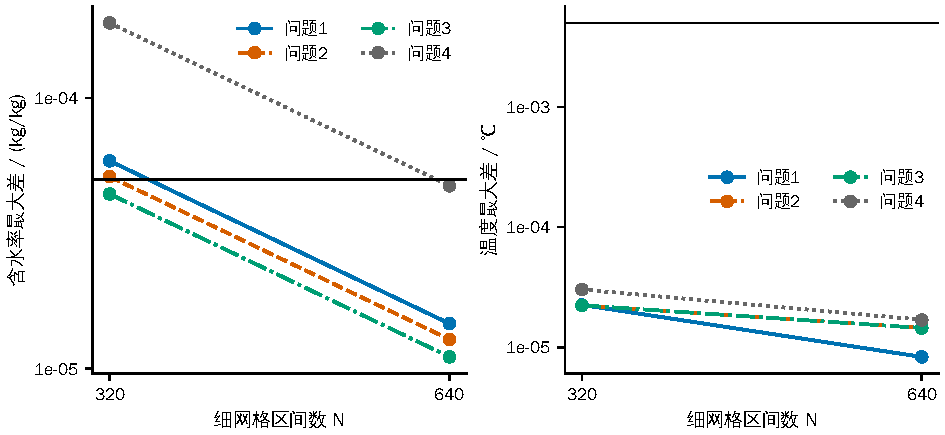
\includegraphics[width=\linewidth]{figures/process_q3_convergence.pdf}
\caption{相邻网格的最大场差，$N$为细网格区间数；横线为含水率与温度误差判据，事件及时间精度结果见表\ref{tab:grid}、\ref{tab:time}。}\label{fig:q3-convergence}
\end{figure}

160至320区间的比较中，问题一、二、四的含水率差超过判据；320至640区间时，全部指标满足要求，故统一采用640区间。含水率差大体降为前一次的四分之一，呈现接近二阶的收敛趋势。

问题三、四在320与640区间下的事件时间分别相差约5.04秒和2.78秒，相对差均小于$10^{-3}$。整秒终点是当前离散模型按严格不等式给出的输出时刻，现有网格比较尚未提供亚秒级绝对误差保证。

\subsection{时间精度与终点稳定性}
在640区间网格上，将相对容差由$10^{-8}$收紧至$10^{-9}$，绝对容差相应收紧，结果见表\ref{tab:time}。四问的最大温度差不超过$1.843\times10^{-5}$摄氏度，最大含水率差不超过$1.589\times10^{-7}$；问题三、四的事件相对差分别为$1.749\times10^{-9}$和$3.510\times10^{-9}$。

\begin{table}[htbp]\centering\small
\caption{最终网格上两组时间容差的差异}\label{tab:time}
\begin{tabular}{crrr}
\toprule
问题 & 最大温度差/摄氏度 & 最大含水率差/(kg/kg) & 事件相对差\\
\midrule
一 & $8.635\times10^{-6}$ & $1.045\times10^{-7}$ & ---\\
二 & $1.476\times10^{-5}$ & $1.295\times10^{-7}$ & ---\\
三 & $1.476\times10^{-5}$ & $1.230\times10^{-7}$ & $1.749\times10^{-9}$\\
四 & $1.842\times10^{-5}$ & $1.589\times10^{-7}$ & $3.510\times10^{-9}$\\
\bottomrule
\end{tabular}
\end{table}

结合表\ref{tab:grid}和表\ref{tab:time}，含水率及终点时间对时间容差的敏感性小于对空间加密的敏感性。温度的两类差异均远低于0.005摄氏度的判据。上述比较支持当前数值设置下的场分布与终点稳定性，误差统计范围均为各检验定义的共同采样点集合。

\section{几何对照与工况灵敏度}
\subsection{分离物性改变与收缩影响}
为考察给定物性下的收缩影响，保持问题四的物性、初值、传递系数及环境延拓不变，仅将半径固定为2厘米。对照越阈时间为129.8449小时，长于收缩情景的51.0908小时。

记$\tau(\mathcal P,R)$为物性组$\mathcal P$和几何轨迹$R$下的越阈时间，$\mathcal P_3$、$\mathcal P_4$分别表示问题三、四的整组物性。现有计算构成$\tau(\mathcal P_3,R_0)\to\tau(\mathcal P_4,R_0)\to\tau(\mathcal P_4,R(t))$的比较路径。先改变物性使时间增加72.3721小时，再引入收缩使时间减少78.7541小时，净变化见式\eqref{eq:path-contrast}。

\begin{equation}\label{eq:path-contrast}
\begin{aligned}
\Delta\tau_{\rm total}
&=\underbrace{\tau(\mathcal P_4,R_0)-\tau(\mathcal P_3,R_0)}_{\text{固定几何下的整组物性差异}}
 +\underbrace{\tau(\mathcal P_4,R(t))-\tau(\mathcal P_4,R_0)}_{\text{问题四物性下的几何差异}}\\
&=72.3721-78.7541\approx-6.3819\ {\rm h}.
\end{aligned}
\end{equation}

差值由未舍入事件时间计算，展示时保留四位小数。沿这条路径，收缩引起的缩短超过整组物性改变引起的延长。该分解依赖所选比较路径，只描述整组物性与给定物性下几何变化的条件差异。

图\ref{fig:q4-counter}比较三种情景，式\eqref{eq:reductions}分别计算总体降幅和同物性下的收缩降幅。前者以问题三为基准，后者以问题四物性、固定半径情景为基准，两个百分比具有不同分母。

\begin{equation}\label{eq:reductions}
\begin{aligned}
\eta_{\rm total}
&=1-\frac{51.090831819}{57.472766796}=11.1043\%,\\
\eta_{\rm shrink}
&=1-\frac{51.090831819}{129.844890064}=60.6524\%.
\end{aligned}
\end{equation}

\begin{figure}[htbp]\centering
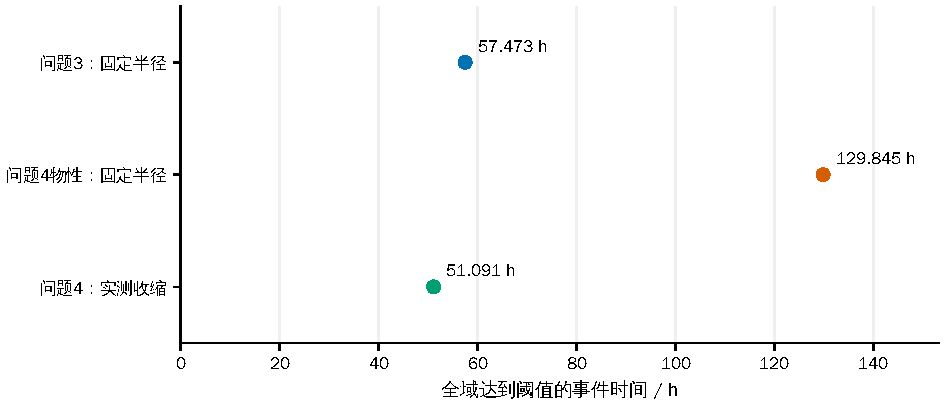
\includegraphics[width=\linewidth]{figures/result_q4_counterfactual.pdf}
\caption{三种情景的越阈时间：上、中两组几何相同，中、下两组物性相同。}\label{fig:q4-counter}
\end{figure}

问题四终点半径约为初始的0.6倍，半径平方约为初始的0.36倍，侧面积与体积之比约增至初始的1.667倍。这些变化分别影响内部扩散尺度和表面交换。实际半径与物性均随过程变化，完成时间由整个变化轨迹上的联立方程确定。

固定半径对照采用独立定义的恒定几何，即使计算超过72小时，也无需延拓收缩记录。该情景继续使用4小时后的恒定环境，用于比较给定物性下的几何影响。

\subsection{环境延拓和传质系数情景}
围绕两问的名义情景，分别采用末值延拓、末小时均值延拓、尾段温度加减0.5摄氏度、尾段有效边界含水率加减0.001以及传质系数加减10\%。环境延拓及温湿扰动从4小时后起作用，传质系数在全过程改变。每次只改变一项设置，越阈时间见表\ref{tab:sensitivity}。

\begin{table}[htbp]\centering\small
\caption{各单因素情景下的全域越阈时间，单位：小时}\label{tab:sensitivity}
\begin{tabular}{lrr}
\toprule
情景 & 问题三 & 问题四\\
\midrule
名义环境及传质系数 & 57.4728 & 51.0908\\
四小时后采用末值 & 57.1698 & 50.8245\\
四小时后采用末小时均值 & 57.4745 & 51.0923\\
尾段温度降低0.5摄氏度 & 58.3959 & 51.9004\\
尾段温度升高0.5摄氏度 & 56.5700 & 50.2989\\
尾段平衡含水率降低0.001 & 57.4532 & 51.0691\\
尾段平衡含水率升高0.001 & 57.4931 & 51.1137\\
全过程传质系数降低10\% & 58.2086 & 51.3820\\
全过程传质系数提高10\% & 56.8954 & 50.8700\\
\bottomrule
\end{tabular}
\end{table}

图\ref{fig:q4-sensitivity}给出相对各自名义时间的变化。尾段温度降低0.5摄氏度时，问题三、四的时间分别增加1.6062\%、1.5846\%；升高时分别减少1.5707\%、1.5500\%。末小时均值延拓与名义情景的差异约为0.003\%，末值延拓约缩短0.52\%。

\begin{figure}[htbp]\centering
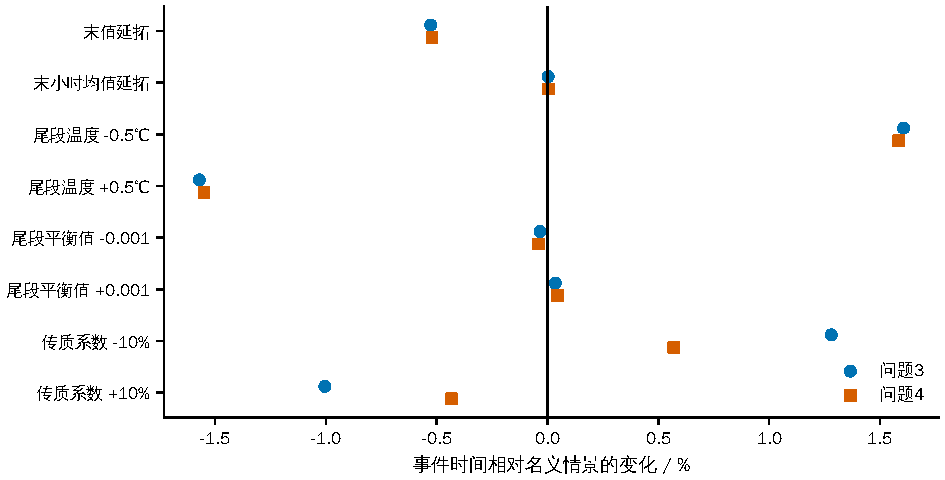
\includegraphics[width=\linewidth]{figures/result_q4_sensitivity.pdf}
\caption{各单因素情景相对本问名义时间的变化，圆点与方块分别表示问题三和问题四。}\label{fig:q4-sensitivity}
\end{figure}

传质系数降低10\%时，问题三、四的时间分别增加1.2804\%、0.5699\%；提高10\%时，分别减少1.0046\%、0.4323\%。在所考察范围内，外部传质条件仍影响完成时间。

各扰动的单位、相对幅度和作用时间不同，结果用于描述所列情景的影响，不能据此给出统一的参数重要性排序或统计置信区间。

在全部已计算的成对情景中，问题四均早于问题三达到阈值，该时间排序在所考察的局部变化下保持一致。

\section{模型评价与适用范围}
\subsection{方法价值及可推广的处理思路}
四问采用共同的状态定义、径向通量离散与终点判据。有限体积法保留柱坐标权重和有限表面交换阻力，随体坐标将均匀收缩纳入同一求解框架。问题二、三共享初边值解，问题四通过更新物性、半径和输出位置描述移动域过程。

最大含水率判据覆盖径向较慢脱水的位置，同物性固定半径对照则区分总体时间差异与几何影响。解析算例、归一化水分收支以及空间和时间加密，从不同方面检验离散方法及终点稳定性。

\subsection{精度、工况与结论边界}
结论适用于表\ref{tab:closure}给出的理想模型。题目未提供内部温度和含水率观测，现有证据支持方程求解的数值一致性，尚缺少与内部观测比较的预测验证。

长期结果还依赖4小时后的环境延拓。所列情景给出了这一约定附近的变化范围，更广泛工况下的结果需按相应边界重新求解。

本题以含水率0.15为完成目标，计算得到温湿场和达标时间。能耗、药效成分及综合品质未作为目标或约束纳入模型。

\section{结论}

采用守恒有限体积法与隐式积分，得到四问的温湿场。问题一在0.50小时的中心、表面温度分别为33.5753、36.7856摄氏度，含水率分别为2.5500、1.5102，明显失水集中在外层。问题二在3小时的径向温差为0.1169摄氏度，中心、表面含水率仍分别为1.7662、1.0081，水分均匀化滞后于升温。

以径向最大含水率低于0.15为完成条件，问题三、四的越阈时间分别为57.4728、51.0908小时，问题四终点半径为1.2000厘米。全过程结果按规定的时间和空间间隔输出，收缩后的域外位置留空。

问题四相对问题三缩短6.3819小时，降幅为11.1043\%。保持问题四物性而固定半径时，对照时间为129.8449小时，同物性下的收缩降幅为60.6524\%。沿先改变整组物性、再引入收缩的比较路径，时间分别增加72.3721小时、减少78.7541小时，解释了最终时间排序。

\section*{AI工具使用声明}
本参赛队在竞赛过程中使用了AI工具，主要用于题意分析、文献线索整理、程序设计与核验、图表制作和文稿编辑，详细使用情况见支撑材料《AI工具使用详情》。

所用工具为OpenAI Codex。本轮由AI将公共模型与各问求解分章整理，编辑摘要和论证文字，核对既有结果并编译检查；未重新计算模型，核心方程和数值结论保留。参赛队最终人工审阅尚待完成，使用者须依据真实记录确认披露，独立理解和核对方程、程序、结果与引用，并对提交内容负责。

\begin{thebibliography}{9}
\small\raggedright
\bibitem{silva2014turmeric}
da Silva W. P., e Silva C. M. D. P. S., Gomes J. P.
Comparison of boundary conditions to describe drying of turmeric
(Curcuma longa) rhizomes using diffusion models[J].
Journal of Food Science and Technology, 2014, 51(11): 3181--3189.
DOI: \href{https://doi.org/10.1007/s13197-012-0813-x}{10.1007/s13197-012-0813-x}.

\bibitem{silva2014coupling}
da Silva W. P., e Silva C. M. D. P. S., Gama F. J. A.
Estimation of thermo-physical properties of products with cylindrical
shape during drying: The coupling between mass and heat[J].
Journal of Food Engineering, 2014, 141: 65--73.
DOI: \href{https://doi.org/10.1016/j.jfoodeng.2014.05.010}{10.1016/j.jfoodeng.2014.05.010}.

\bibitem{tzempelikos2015quince}
Tzempelikos D. A., Mitrakos D., Vouros A. P., Bardakas A. V.,
Filios A. E., Margaris D. P.
Numerical modeling of heat and mass transfer during convective
drying of cylindrical quince slices[J].
Journal of Food Engineering, 2015, 156: 10--21.
DOI: \href{https://doi.org/10.1016/j.jfoodeng.2015.01.017}{10.1016/j.jfoodeng.2015.01.017}.

\bibitem{seyedabadi2017ale}
Seyedabadi E., Khojastehpour M., Abbaspour-Fard M. H.
Convective drying simulation of banana slabs considering non-isotropic
shrinkage using FEM with the Arbitrary Lagrangian--Eulerian method[J].
International Journal of Food Properties, 2017, 20(sup1): S36--S49.
DOI: \href{https://doi.org/10.1080/10942912.2017.1288134}{10.1080/10942912.2017.1288134}.

\bibitem{adrover2020pears}
Adrover A., Venditti C., Brasiello A.
A Non-Isothermal Moving-Boundary Model for Continuous and
Intermittent Drying of Pears[J].
Foods, 2020, 9(11): 1577.
DOI: \href{https://doi.org/10.3390/foods9111577}{10.3390/foods9111577}.
\end{thebibliography}

\clearpage
\appendix
\section{支撑材料文件清单}\label{app:materials}
表\ref{tab:catalog}列出当前支撑材料文件及用途。工作区根目录的“答案”文件夹集中保存题目要求填写的四个结果工作簿；其余材料位于“A题/论文提升\_20260913\_v4/”工程目录，表中其余路径均相对于该工程目录。附录B给出七个脚本、五个辅助模块及依赖清单。

\begin{table}[htbp]\centering\small
\caption{电子支撑材料目录}\label{tab:catalog}
\begin{tabularx}{\linewidth}{lX}
\toprule
文件或目录 & 内容\\
\midrule
答案 & \texttt{result1.xlsx}、\texttt{result2.xlsx}、\texttt{result3.xlsx}、\texttt{result4.xlsx}，分别对应问题一至四的已填写结果，与\texttt{results/}中的同名文件一致\\
\texttt{solve.py} & 物性、网格、通量、雅可比、积分、事件与小算例检验\\
\texttt{run\_all.py} & 网格和时间复验、结果表、场数组及情景分析\\
\texttt{make\_figures.py} & 从真实结果生成14组矢量和位图\\
\texttt{verify\_moving\_domain.py} & 移动域解析模态、时空加密、几何因子对照与守恒检验\\
\texttt{export\_result2\_full.py} & 全过程逐秒工作簿的分块导出和完整结构检查\\
\texttt{reproduce.py} & 完整计算、验证和导出的运行入口\\
\texttt{test\_sync.py} & 采样统计与600 s导出的短程检查\\
\texttt{utils/} & 全量读表、绘图风格、图表自检、导出与环境记录\\
\texttt{requirements.txt} & 原计算使用的Python包版本\\
\texttt{results/} & 四个结果工作簿的原始输出、六张题表、全过程时空输出、过程数组、域外空值规则、诊断与参数摘要\\
\texttt{figures/} & 原始输入、运行过程和结果图的PDF、SVG、PNG\\
新增示意图/ & 三张框架、流程与随体坐标图的可编辑源文件和矢量插入版本\\
完整论文-LaTeX/ & 主文稿、章节、表格、图形及完整代码副本\\
AI工具使用详情.pdf & 关键提示、采纳范围、工具说明和人工复核提示\\
AI工具说明-LaTeX/ & AI工具使用说明的LaTeX源码与配图\\
\bottomrule
\end{tabularx}
\end{table}

计算环境为Python 3.10.12，包版本见\texttt{requirements.txt}。准备依赖及文泉驿正黑字体\texttt{wqy-zenhei.ttc}后，从包含原始附件的项目根目录执行：
\begin{Verbatim}[fontsize=\small,breaklines,breakanywhere]
OPENBLAS_NUM_THREADS=1 OMP_NUM_THREADS=1 python3 -B reproduce.py
\end{Verbatim}

完整入口在\texttt{reproduced\_*}目录依次计算解析基准、四问结果、空间与时间精度比较、工作簿、情景对照和图形，保留原有结果。需要短程检查或单独运行移动域算例时，可分别使用：
\begin{Verbatim}[fontsize=\small,breaklines,breakanywhere]
python3 -B reproduce.py --smoke
python3 -B verify_moving_domain.py
python3 -B verify_moving_domain.py --mutant-only
\end{Verbatim}

\section{完整可运行源代码}

\subsection{核心求解与诊断}
\VerbatimInput[fontsize=\scriptsize,breaklines,breakanywhere,breaksymbolleft={},breaksymbolright={},frame=single,framerule=0.4pt,framesep=2mm]{code/solve.py}
\subsection{全流程计算与结果导出}
\VerbatimInput[fontsize=\scriptsize,breaklines,breakanywhere,breaksymbolleft={},breaksymbolright={},frame=single,framerule=0.4pt,framesep=2mm]{code/run_all.py}
\subsection{真实结果可视化}
\VerbatimInput[fontsize=\scriptsize,breaklines,breakanywhere,breaksymbolleft={},breaksymbolright={},frame=single,framerule=0.4pt,framesep=2mm]{code/make_figures.py}
\subsection{移动域解析基准与几何因子对照}
\VerbatimInput[fontsize=\scriptsize,breaklines,breakanywhere,breaksymbolleft={},breaksymbolright={},frame=single,framerule=0.4pt,framesep=2mm]{code/verify_moving_domain.py}
\subsection{全过程逐秒工作簿导出与核对}
\VerbatimInput[fontsize=\scriptsize,breaklines,breakanywhere,breaksymbolleft={},breaksymbolright={},frame=single,framerule=0.4pt,framesep=2mm]{code/export_result2_full.py}
\subsection{完整计算入口}
\VerbatimInput[fontsize=\scriptsize,breaklines,breakanywhere,breaksymbolleft={},breaksymbolright={},frame=single,framerule=0.4pt,framesep=2mm]{code/reproduce.py}
\subsection{采样与导出检查}
\VerbatimInput[fontsize=\scriptsize,breaklines,breakanywhere,breaksymbolleft={},breaksymbolright={},frame=single,framerule=0.4pt,framesep=2mm]{code/test_sync.py}
\subsection{完整附件读取}
\VerbatimInput[fontsize=\scriptsize,breaklines,breakanywhere,breaksymbolleft={},breaksymbolright={},frame=single,framerule=0.4pt,framesep=2mm]{code/utils/read_rows.py}
\subsection{图表结构与布局检查}
\VerbatimInput[fontsize=\scriptsize,breaklines,breakanywhere,breaksymbolleft={},breaksymbolright={},frame=single,framerule=0.4pt,framesep=2mm]{code/utils/plot_style.py}
\subsection{统一科研绘图风格}
\VerbatimInput[fontsize=\scriptsize,breaklines,breakanywhere,breaksymbolleft={},breaksymbolright={},frame=single,framerule=0.4pt,framesep=2mm]{code/utils/setup_style.py}
\subsection{多格式图表导出}
\VerbatimInput[fontsize=\scriptsize,breaklines,breakanywhere,breaksymbolleft={},breaksymbolright={},frame=single,framerule=0.4pt,framesep=2mm]{code/utils/export_figure.py}
\subsection{输入与运行环境记录}
\VerbatimInput[fontsize=\scriptsize,breaklines,breakanywhere,breaksymbolleft={},breaksymbolright={},frame=single,framerule=0.4pt,framesep=2mm]{code/utils/repro_manifest.py}
\subsection{Python依赖版本}
\VerbatimInput[fontsize=\small,breaklines,frame=single,framerule=0.4pt,framesep=2mm]{code/requirements.txt}

\end{document}
